\documentclass[referee,lineno,pdflatex,sn-apa]{sn-jnl}

\usepackage{graphicx}
\usepackage{booktabs}
\usepackage{multirow}
\usepackage{amsmath,amssymb}
\usepackage{xcolor}
\usepackage{url}

\graphicspath{{figures/}}
\raggedbottom

\begin{document}

\title[Terrain-Conditioned Avalanche Mapping]{Terrain-Conditioned Cross-Attention for Cross-Region Avalanche Debris Mapping with Sentinel-1 SAR}

% Double-blind manuscript: author information is supplied in a separate title page.
\author[1]{\fnm{}\sur{}}
\affil[1]{\orgname{Author affiliations withheld for double-blind peer review}}

\abstract{Cloud cover, winter darkness, and steep terrain complicate regional mapping of avalanche debris. Sentinel-1 synthetic aperture radar (SAR) provides all-weather observations, but slope-dependent foreshortening, layover, and shadow can resemble bitemporal change. We present TopoRadar-Net, a lightweight change-segmentation model that conditions SAR features on local incidence angle, slope, aspect, elevation, and a fixed-reference aspect coordinate through multiscale cross-attention. We evaluate five architectures on AvalCD, comprising seven events, four mountain systems, and 993 avalanche polygons. Models are trained on Alps and Greenland scenes and tested without site-specific tuning in Troms{\o} and the Pamirs. Across three seeds, TopoRadar-Net obtains $63.79\% \pm 1.88\%$ pooled macro F1 (mean $\pm$ population standard deviation). Its margin over a bottleneck self-attention U-Net is $+0.38$ percentage points ($p=0.869$), whereas its margin over SiamUNet-diff is $+8.92$ percentage points ($p=0.021$). Ablations show regional rather than uniform benefits: removing aspect conditioning or cross-attention increases pooled F1, while the slope prior overlaps $18.47\%$ of training positives. A validation-calibrated road-corridor proxy reaches $83.0\%$ precision and $62.5\%$ recall in the Pamirs but misses the single Troms{\o} corridor avalanche in every seed. Terrain conditioning is therefore competitive and diagnostically useful, but not uniformly superior or deployment-ready.}

\keywords{Sentinel-1 SAR, snow avalanche mapping, semantic segmentation, radar geometry, cross-region evaluation, deep learning}

\maketitle

\section{Introduction}

Regional avalanche-debris maps support event documentation, hazard assessment, and prioritization of field inspection. Optical observations are often unavailable during major winter storms, while Sentinel-1 C-band synthetic aperture radar (SAR) supplies day-and-night measurements through cloud cover \citep{eckerstorfer2017remote,eckerstorfer2019near,muller2021synthetic}. Avalanche deposits roughen the snow surface and can increase post-event co- and cross-polarized backscatter, making bitemporal change detection useful \citep{tompkin2021backscatter}. AvalCD supplies VV/VH for Livigno, Troms{\o}, and Pish, but HH/HV for Nuuk. Side-looking geometry also produces slope-dependent foreshortening, layover, shadow, and radiometric variation that can resemble debris.

Recent remote-sensing studies show that deep learning can map slope hazards across diverse environments, but shadows, scale changes, class imbalance, and geographic transfer remain difficult \citep{nguyen2025landslide,chandra2025landslide}. SAR-specific segmentation and change-image construction introduce additional representation choices \citep{arjasakusuma2024sar,wang2025change}. In the same hazard domain, \citet{ahmad2026avalanche} model pre-event avalanche susceptibility with attention, whereas our target is post-event debris. Debris mapping for emergency response also needs explicit comparison and operationally meaningful validation rather than accuracy alone \citep{bayat2026debris}.

The closest avalanche-segmentation precedents already contain terrain conditioning. \citet{bianchi2021snow} apply a potential-angle-of-reach-conditioned attention mask and slope feature map to Sentinel-1 avalanche segmentation. On AvalCD, \citet{gatti2026avalanche} encode local incidence angle and slope in a separate transformer branch and report that SAR-only change detection is more consistent than terrain-augmented variants. Concurrently, \citet{gelato2026promptable} adapt a promptable foundation model to SAR avalanche segmentation using SAR, elevation, and slope inputs and evaluate annotation-time reduction. Our target instead is autonomous bitemporal change segmentation across held-out regions, with multi-seed failure characterization rather than prompt-driven annotation. Our architectural delta is narrower: SAR-change queries attend to pooled terrain keys and values, including a fixed $78^\circ$ aspect-reference channel. The empirical contribution is the three-seed, leave-region-out characterization of component instability, positive-label conflict in the slope prior, and a bounded corridor proxy---not a claim that terrain conditioning uniformly improves accuracy.

We evaluate whether radar-topographic conditioning improves avalanche change segmentation across unseen mountain systems. TopoRadar-Net uses bitemporal SAR differences as queries and multiscale terrain geometry as keys and values. The study contributes: (1) a compact terrain-conditioned cross-attention architecture; (2) three-seed zero-shot evaluation against four baselines on two held-out mountain systems; (3) spatial-block inference, component ablations, and terrain-stratum stability checks; and (4) construct and corridor audits that expose where the model should not be interpreted operationally. The objective is not to claim uniform superiority, but to establish where terrain conditioning changes performance and where its assumptions fail.

\section{Data and Study Design}

AvalCD contains co-registered pre/post-event Sentinel-1 intensity, topography, valid-data masks, and expert-mapped avalanche polygons \citep{gatti2026avalanche,avalcd_dataset}. The seven events span the European Alps, Greenland Arctic, Scandinavian Arctic, and Pamir Mountains (Table~\ref{tab:data}). Livigno events from April 2024 and January 2025 plus Nuuk 2016 form the training cohort. Livigno March 2025 and Nuuk 2021 are used for validation, checkpoint selection, and decision-threshold calibration. Troms{\o} 2024 and Pish 2023 remain geographically held out for final testing. This split changes climate, relief, polarization regime, acquisition geometry, and avalanche morphology simultaneously; results quantify cross-system transfer but do not identify any one changed factor as causal.

\begin{table}[t]
\caption{AvalCD scenes used in the cross-region study. Debris is the number of labelled positive pixels}
\label{tab:data}
\centering
\scriptsize
\begin{tabular}{lllllrr}
\toprule
System & Scene date & Role & Region & Pol. & Polygons & Debris \\
\midrule
Alps & 3 Apr 2024 & Train & Livigno & VV/VH & 231 & 32,606 \\
Alps & 29 Jan 2025 & Train & Livigno & VV/VH & 207 & 11,438 \\
Alps & 18 Mar 2025 & Validate & Livigno & VV/VH & 79 & 7,392 \\
Greenland & 13 Apr 2016 & Train & Nuuk & HH/HV & 117 & 64,822 \\
Greenland & 11 Apr 2021 & Validate & Nuuk & HH/HV & 129 & 81,595 \\
Pamirs & 21 Feb 2023 & Test & Pish & VV/VH & 113 & 22,579 \\
Scand. Arctic & 20 Dec 2024 & Test & Troms{\o} & VV/VH & 117 & 33,972 \\
\bottomrule
\end{tabular}
\end{table}

The executed loader uses the supplied decibel rasters without percentile scaling. Values outside $[-45,15]$ dB are marked invalid; after the valid mask is fixed, missing cross- and co-polarized values are replaced by $-20$ and $-12$ dB, respectively. The two model positions represent cross/co polarization (VH/VV or HV/HH according to scene), and difference channels retain those positions. The terrain tensor contains local incidence angle (LIA), slope, sine/cosine aspect, elevation from a digital elevation model (DEM), and the fixed coordinate $\cos(\alpha-78^\circ)$; this last channel is a reference-axis aspect encoding, not authoritative per-event radar heading. Training uses balanced $128\times128$ patches; evaluation uses complete valid-mask rasters. Physical areas are derived from affine raster transforms rather than full rectangular extents. Figure~\ref{fig:architecture} summarizes the model; Online Resource~1 supplies equations, preprocessing details, complete tables, and additional diagnostics.

\section{Method}

\subsection{Radar-topographic conditioning}

Let $I^{\mathrm{pre}}$ and $I^{\mathrm{post}}$ denote pre- and post-event two-channel cross/co-polarized intensity tensors. A shared residual encoder produces scale-$l$ features $F_l^{\mathrm{pre}}$ and $F_l^{\mathrm{post}}$. Their difference representation is
\begin{equation}
F_l^{\Delta}=\operatorname{Conv}\!\left[
F_l^{\mathrm{post}}-F_l^{\mathrm{pre}},
F_l^{\mathrm{post}},
F_l^{\mathrm{pre}}\right].
\end{equation}
The terrain encoder maps the six-channel geometry tensor to $T_l$. A Radar-Topographic Cross-Attention Block (RTCAB) forms SAR queries and pooled terrain keys and values,
\begin{equation}
Q=F_l^{\Delta}W_Q,\quad K=\operatorname{Pool}(T_l)W_K,\quad
V=\operatorname{Pool}(T_l)W_V,
\end{equation}
and computes $A=\operatorname{softmax}(QK^\top/\sqrt{d})V$. A pixelwise gate $\sigma(\operatorname{Conv}(T_l))$ modulates the attended features before progressive decoding. This construction conditions a shift-invariant convolutional representation on spatially varying radar geometry; it does not make the representation physically invariant.

\begin{figure}[t]
\centering
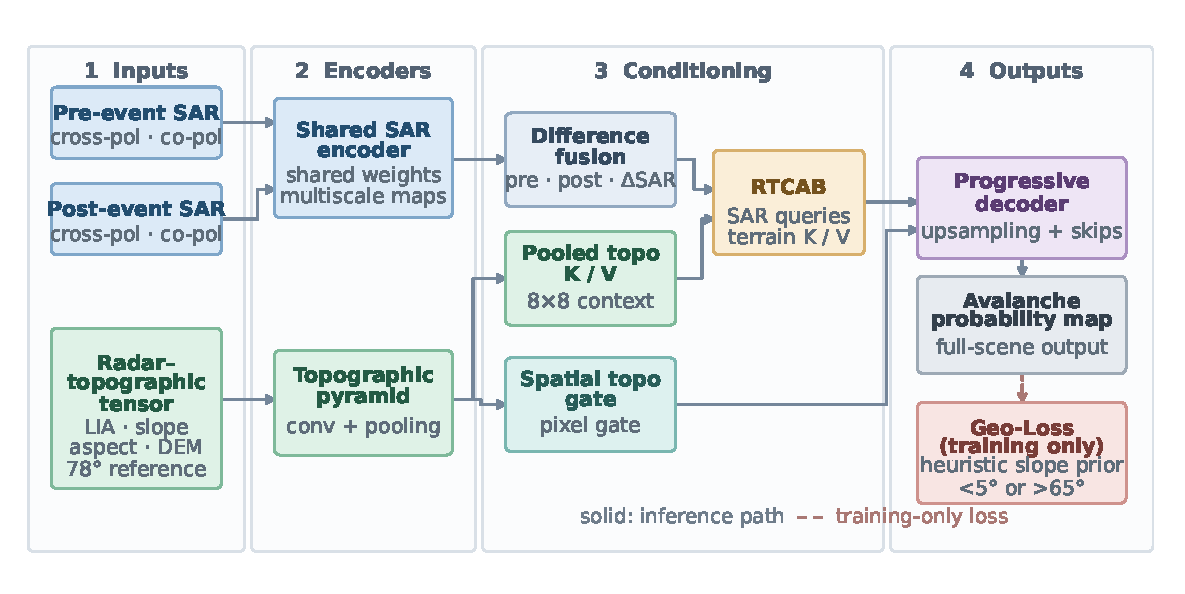
\includegraphics[width=\textwidth]{Fig1.pdf}
\caption{TopoRadar-Net schematic. Bitemporal SAR differences query pooled topographic keys and values; a pixelwise terrain gate conditions decoding. The training schematic omits the ground-truth loss input for clarity}
\label{fig:architecture}
\end{figure}

\subsection{Loss, training, and inference}

The objective combines positive-weighted binary cross-entropy (BCE), Dice loss, and a soft slope prior:
\begin{equation}
\mathcal{L}=\mathcal{L}_{\mathrm{BCE}}+\mathcal{L}_{\mathrm{Dice}}+0.5\,\mathcal{L}_{\mathrm{slope}}.
\end{equation}
The prior discourages probability mass below $5^\circ$ and above $65^\circ$ but is treated as a heuristic because mapped positives occur in this mask. All models use the same optimizer, six-epoch schedule, balanced patches, validation-selected checkpoint, and full-scene threshold calibration. We train fixed seeds 42, 123, and 456. Comparators are SiamUNet-diff and SiamUNet-conc \citep{daudt2018fully}, ResU-Net \citep{zhang2018road}, and an internal bottleneck self-attention U-Net. The internal baseline uses the same convolutional encoder--decoder scale with four-head self-attention only at the deepest feature map; it is neither canonical attention-gated U-Net nor Swin-UNet. Parameter counts range from 2.01 to 3.46 million.

Inference uses overlapping windows with Hanning blending. Pixel F1 and intersection-over-union are computed over valid pixels. Polygon hit rate requires at least $30\%$ overlap. A 1,000-draw paired bootstrap resamples $128\times128$ spatial blocks; paired seed-level tests use the three macro-F1 values. The latter have low power and are interpreted together with effect sizes and ordering across seeds. No test pixel or test label is used for model or threshold selection.

For a post-hoc operational proxy, validation-scene component scores calibrate a one-feature logistic model and an F2-optimal alert threshold. Frozen test-scene alerts are intersected with 30-m buffers around a versioned OpenStreetMap major-road snapshot \citep{openstreetmap2026}. This retrospective proxy excludes data acquisition, human review, dispatch, and closure decisions. Figures~\ref{fig:architecture} and \ref{fig:performance} were generated with Python 3.14.7 and Matplotlib 3.11.2.

\subsection{AI-assisted research support}

Generative AI tools assisted code refactoring, manuscript language, and checklist-based consistency checking. They did not generate research data or determine final scientific claims. The authors inspected generated material, reran the analysis and verification code, checked citations and numerical statements, and retain full responsibility for the work.

\section{Results}

\subsection{Cross-region performance}

TopoRadar-Net records $77.40\%\pm1.86\%$ F1 in Troms{\o} and $50.18\%\pm4.40\%$ in Pish, giving $63.79\%\pm1.88\%$ pooled macro F1 (Table~\ref{tab:performance}). The bottleneck self-attention U-Net obtains $63.41\%\pm1.03\%$, SiamUNet-conc $63.13\%\pm0.79\%$, and ResU-Net $62.92\%\pm1.42\%$. Their differences from TopoRadar-Net are not significant across three seeds. SiamUNet-diff is lower at $54.87\%\pm1.03\%$; the paired difference is $+8.92$ percentage points (95\% confidence interval [CI] $+3.25$ to $+14.59$, $p=0.021$). The bottleneck self-attention U-Net leads on seed 123, demonstrating initialization-dependent ordering. Figure~\ref{fig:performance} visualizes the region-specific ordering.

\begin{table}[t]
\caption{Zero-shot test performance across three fixed training seeds (mean $\pm$ descriptive population standard deviation). HR is polygon hit rate at $30\%$ overlap}
\label{tab:performance}
\centering
\small
\begin{tabular}{lrrrr}
\toprule
Method & Troms{\o} F1 & Pish F1 & Pooled F1 & Troms{\o} HR \\
\midrule
SiamUNet-diff & $72.64\pm0.39$ & $37.11\pm2.44$ & $54.87\pm1.03$ & $63.25\pm2.52$ \\
SiamUNet-conc & $78.92\pm1.07$ & $47.34\pm0.70$ & $63.13\pm0.79$ & $82.62\pm1.07$ \\
ResU-Net & $76.60\pm1.30$ & $49.25\pm3.39$ & $62.92\pm1.42$ & $76.92\pm4.83$ \\
Self-attention U-Net & $78.09\pm0.99$ & $48.73\pm2.74$ & $63.41\pm1.03$ & $79.20\pm2.45$ \\
TopoRadar-Net & $77.40\pm1.86$ & $50.18\pm4.40$ & $63.79\pm1.88$ & $75.50\pm1.61$ \\
\bottomrule
\end{tabular}
\end{table}

\begin{figure}[t]
\centering
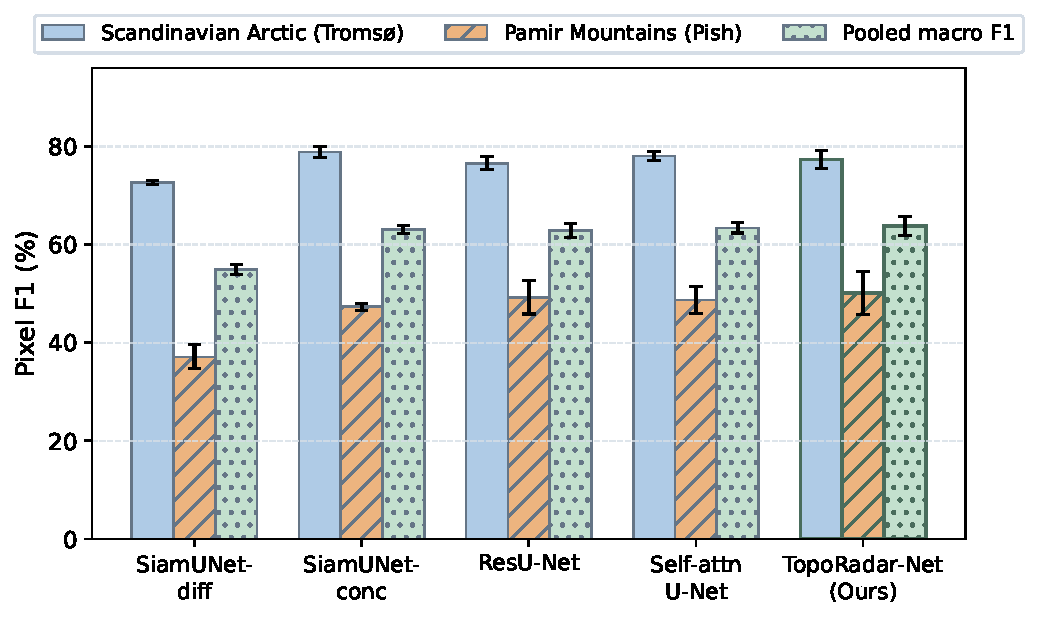
\includegraphics[width=0.95\textwidth]{Fig2.pdf}
\caption{Zero-shot pixel F1 across held-out Troms{\o}, Pish, and their macro average. Error bars show descriptive population standard deviation over three fixed training seeds}
\label{fig:performance}
\end{figure}

The 339-block seed-42 bootstrap gives a $+3.27$-percentage-point micro-F1 difference from the self-attention U-Net (95\% CI $+1.12$ to $+5.37$, $p=0.010$), but repeating the bootstrap by training seed yields $+3.26$, $-2.99$, and $+4.16$ percentage points. Thus a conditional spatial interval is not a substitute for training uncertainty. On the Nuuk validation scene, all modern architectures lie within 0.63 F1 percentage points, providing additional evidence of parity rather than uniform dominance.

Online Resource~1 reports polygon completeness by European Avalanche Warning Services destructive-size classes \citep{eaws2022size}; these classes are available for Troms{\o} but not Pish.

\subsection{Component sensitivity and failure boundaries}

The full architecture is not the best pooled configuration (Table~\ref{tab:ablation}). Removing aspect and its fixed-reference coordinate or removing cross-attention increases pooled macro F1 to $65.35\%$ and $65.07\%$, respectively, mainly through gains in Pish. In Troms{\o}, seed-42 paired block tests favour the full model over No-LIA by $2.04$ percentage points ($p<0.001$) and No-CrossAttn by $1.42$ percentage points ($p=0.010$). These comparisons establish component sensitivity, not a causal terrain-correction mechanism.

\begin{table}[t]
\caption{Ablation performance across three seeds. The highest pooled value is obtained without aspect and its fixed-reference coordinate}
\label{tab:ablation}
\centering
\small
\begin{tabular}{lrrr}
\toprule
Configuration & Troms{\o} F1 & Pish F1 & Pooled F1 \\
\midrule
Full & $77.40\pm1.86$ & $50.18\pm4.40$ & $63.79\pm1.88$ \\
No local incidence angle & $75.67\pm1.76$ & $52.13\pm1.11$ & $63.90\pm1.37$ \\
No cross-attention & $76.85\pm0.80$ & $53.30\pm0.93$ & $65.07\pm0.53$ \\
No slope prior & $76.70\pm0.91$ & $51.99\pm1.31$ & $64.35\pm1.05$ \\
No aspect/reference coordinate & $77.38\pm2.66$ & $53.32\pm0.42$ & $65.35\pm1.54$ \\
\bottomrule
\end{tabular}
\end{table}

The slope-prior mask contains $18.47\%$ of valid training positives, $0.95\%$ of validation positives, and $0.87\%$ of held-out positives. Within the held-out penalty stratum, the full model has lower three-seed positive recall than No-GeoLoss in Troms{\o} ($50.47\%\pm3.18\%$ versus $71.29\%\pm6.39\%$) and Pish ($1.08\%\pm1.52\%$ versus $6.45\%\pm6.97\%$). The term is therefore a precision--recall prior, not a physical-admissibility rule.

Seed-42 terrain strata initially suggest positive backslope differences, but these do not persist across seeds: TopoRadar-Net minus the self-attention U-Net averages $-0.34\%\pm6.28\%$ in Troms{\o} and $+1.20\%\pm7.73\%$ in Pish. Extreme-steep terrain is highly variable and both models perform poorly in the small Pish shadow stratum. Complete stratum results are in Online Resource~1.

\subsection{Retrospective corridor proxy}

The affine valid-mask area is $196.820~\mathrm{km}^{2}$ in Troms{\o} and $267.435~\mathrm{km}^{2}$ in Pish. In Troms{\o}, TopoRadar-Net produces $74.77$ ha of false positives at $0.38~\mathrm{ha\,km}^{-2}$. In Pish, it produces $129.69$ ha at $0.48~\mathrm{ha\,km}^{-2}$. Relative to the self-attention U-Net, this is a 30.0\% reduction in Pish (129.69 versus 185.32 ha) but a 28.5\% increase in Troms{\o} (74.77 versus 58.19 ha). Validation-calibrated road-corridor alerts achieve $83.0\%$ precision and $62.5\%$ recall in Pish. The single road-intersecting reference avalanche in Troms{\o} is missed by every TopoRadar-Net seed. All cached complete-scene runs are below 5 s on Apple Metal Performance Shaders hardware, but timing excludes upstream acquisition and human review.

\section{Discussion}

TopoRadar-Net is competitive across unseen mountain systems, but the strongest baselines are statistically indistinguishable across three seeds. This result is important for remote-sensing model design: adding physically interpretable variables does not guarantee a better predictor. Recent hazard-mapping studies similarly motivate multiscale or attention modules across diverse environments \citep{nguyen2025landslide,chandra2025landslide}, while our cross-region ablations show that auxiliary geometry can reverse model ordering. The contribution is therefore the controlled characterization of terrain conditioning under geographic shift, including evidence against a uniform advantage.

The construct audit changes the interpretation of the slope loss. Genuine positives inside the penalty mask arise through runout, raster alignment, and terrain-model uncertainty; suppressing them can increase precision while reducing recall. A hard ``impossible terrain'' label would be unsupported. Likewise, seed-42 terrain-stratum differences are descriptive because seed repetition does not preserve their magnitude or sign.

Operationally, the component and corridor analyses resemble recent efforts to connect mapped debris with transport access \citep{bayat2026debris}, but they remain retrospective. The Pish corridor result is encouraging; the Troms{\o} miss falsifies any claim of region-independent completeness. Prospective evaluation with warning services or road authorities must measure acquisition delay, review burden, missed-event cost, and decision outcomes before deployment.

Limitations include seven events from one benchmark, three training seeds, correlated spatial blocks, threshold calibration on only two scenes, incomplete event metadata for size analysis outside Troms{\o}, and the non-equivariant directional augmentation inherited by the released checkpoints. Sentinel-1 C-band also has an irreducible shadow boundary in very steep relief. Future validation in the Indian Himalaya would be valuable, but this study contains no Indian test data and makes no India-specific accuracy claim. Application to RISAT or NISAR would require sensor-specific calibration and independent Himalayan labels.

\section{Conclusion}

Terrain-conditioned cross-attention provides competitive Sentinel-1 avalanche-debris segmentation and useful failure diagnostics, but it is not uniformly superior to standard change networks. TopoRadar-Net reaches $63.79\%$ pooled macro F1 across two unseen mountain systems; only its margin over SiamUNet-diff is significant across seeds. Aspect and cross-attention ablations improve pooled F1, and the slope prior suppresses genuine positives. The corridor proxy succeeds in Pish but fails on the only Troms{\o} corridor event. The defensible conclusion is therefore bounded: radar-topographic conditioning can alter regional precision and recall, while cross-region reliability still requires explicit validation.

\section*{Data Availability/Supplementary Information}

The AvalCD benchmark is publicly available at \url{https://doi.org/10.5281/zenodo.15863589}. \textbf{Online Resource 1.} Extended methods, complete statistical and subgroup results, and reproducibility identifiers. Code and checkpoint files are publicly archived; the identifying repository URL is withheld from the anonymous manuscript and supplied separately to the editorial office for double-blind review.

\section*{Statements and Declarations}

\textbf{Funding.} No external grant funding was received for this study.

\textbf{Competing interests.} The authors declare no competing financial or non-financial interests.

\textbf{Ethics approval and consent.} Not applicable; the study uses public remote-sensing data and contains no human participants or animals.

\textbf{Consent for publication.} Not applicable.

\textbf{Author contributions.} The complete CRediT statement is provided on the separate title page.

\textbf{AI disclosure.} Generative AI assistance is documented in the Methods section. The authors retain responsibility for all code, analyses, citations, and text.

\bibliography{references}

\end{document}
